\documentclass{beamer}
\usepackage[utf8]{inputenc}
\usepackage{graphicx, epsfig}
\usepackage{amsmath,mathrsfs,amsfonts,amssymb}
\usepackage{floatflt}
\usepackage{epic,ecltree}
\usepackage{mathtext}
\usepackage{fancybox}
\usepackage{fancyhdr}
\usepackage{multirow}
\usepackage{enumerate}
\usepackage{epstopdf}
\usepackage{multicol}
\usepackage{algorithm}
\usepackage[noend]{algorithmic}
\usepackage{tikz}
\usepackage{blindtext}
\usetheme{default}%{Singapore}%{Warsaw}%{Warsaw}%{Darmstadt}
\usecolortheme{default}

\setbeamerfont{title}{size=\Huge}
\setbeamertemplate{footline}[page number]{}

\setbeamertemplate{section in toc}[sections numbered]


\makeatletter
\newcommand\HUGE{\@setfontsize\Huge{35}{40}}
\makeatother    

\setbeamerfont{title}{size=\HUGE}
\beamertemplatenavigationsymbolsempty

% latin bold lower
\newcommand{\ba}{\mathbf{a}} 
\newcommand{\bc}{\mathbf{c}} 
\newcommand{\be}{\mathbf{e}} 
\newcommand{\bh}{\mathbf{h}} 
\newcommand{\bp}{\mathbf{p}} 
\newcommand{\bt}{\mathbf{t}} 
\newcommand{\bs}{\mathbf{s}} 
\newcommand{\bu}{\mathbf{u}} 
\newcommand{\bv}{\mathbf{v}} 
\newcommand{\bw}{\mathbf{w}} 
\newcommand{\bx}{\mathbf{x}} 
\newcommand{\by}{\mathbf{y}} 
\newcommand{\bz}{\mathbf{z}} 

% latin bold upper
\newcommand{\bA}{\mathbf{A}} 
\newcommand{\bB}{\mathbf{B}} 
\newcommand{\bC}{\mathbf{C}} 
\newcommand{\bI}{\mathbf{I}} 
\newcommand{\bJ}{\mathbf{J}} 
\newcommand{\bL}{\mathbf{L}} 
\newcommand{\bM}{\mathbf{M}} 
\newcommand{\bP}{\mathbf{P}}
\newcommand{\bQ}{\mathbf{Q}} 
\newcommand{\bR}{\mathbf{R}} 
\newcommand{\bT}{\mathbf{T}} 
\newcommand{\bU}{\mathbf{U}} 
\newcommand{\bV}{\mathbf{V}} 
\newcommand{\bW}{\mathbf{W}} 
\newcommand{\bX}{\mathbf{X}} 
\newcommand{\bY}{\mathbf{Y}} 
\newcommand{\bZ}{\mathbf{Z}} 

% latin cal upper
\newcommand{\cF}{\mathcal{F}} 
\newcommand{\cG}{\mathcal{G}} 
\newcommand{\cI}{\mathcal{I}} 
\newcommand{\cL}{\mathcal{L}} 
\newcommand{\cM}{\mathcal{M}} 
\newcommand{\cN}{\mathcal{N}} 
\newcommand{\cS}{\mathcal{S}} 
\newcommand{\cT}{\mathcal{T}} 
\newcommand{\cW}{\mathcal{W}} 
\newcommand{\cX}{\mathcal{X}} 
\newcommand{\cZ}{\mathcal{Z}} 

% latin bb upper
\newcommand{\bbE}{\mathbb{E}} 
\newcommand{\bbI}{\mathbb{I}} 
\newcommand{\bbP}{\mathbb{P}} 
\newcommand{\bbR}{\mathbb{R}} 

% greek bold lower
\newcommand{\bepsilon}{\boldsymbol{\epsilon}} 
\newcommand{\btheta}{\boldsymbol{\theta}} 
\newcommand{\blambda}{\boldsymbol{\lambda}} 
\newcommand{\bpi}{\boldsymbol{\pi}} 
\newcommand{\bmu}{\boldsymbol{\mu}} 
\newcommand{\bsigma}{\boldsymbol{\sigma}} 
\newcommand{\bphi}{\boldsymbol{\phi}} 

% greek bold upper
\newcommand{\bSigma}{\boldsymbol{\Sigma}} 

\DeclareMathOperator*{\argmin}{arg\,min}
\DeclareMathOperator*{\argmax}{arg\,max}

\newcommand{\createdgmtitle}[1]{\title[\hbox to 56mm{Deep Generative Models  \hfill\insertframenumber\,/\,\inserttotalframenumber}]
	{\vspace{1cm} \\ Deep Generative Models \\ {\Huge Lecture #1}}
	\author{Roman Isachenko}
	\institute{
	Moscow Institute of Physics and Technology
	} 
	\date{2023, Autumn}
}

\usepackage{tikz}
\usetikzlibrary{arrows,shapes,positioning,shadows,trees}

\newcommand\myfootnote[1]{%
  \tikz[remember picture,overlay]
  \draw (current page.south west) +(1in + \oddsidemargin,0.5em)
  node[anchor=south west,inner sep=0pt]{\parbox{\textwidth}{%
      \rlap{\rule{10em}{0.4pt}}\raggedright\scriptsize \textit{#1}}};}

\newcommand\myfootnotewithlink[2]{%
  \tikz[remember picture,overlay]
  \draw (current page.south west) +(1in + \oddsidemargin,0.5em)
  node[anchor=south west,inner sep=0pt]{\parbox{\textwidth}{%
      \rlap{\rule{10em}{0.4pt}}\raggedright\scriptsize\href{#1}{\textit{#2}}}};}
      
\AtBeginSection[]
      {
      	\begin{frame}{Outline}
      		\tableofcontents[currentsection]
      	\end{frame}
      }
      \AtBeginSubsection[]{
      	\begin{frame}{Outline}
      		\tableofcontents[currentsection,currentsubsection]
      	\end{frame}
}
\createdgmtitle{6}
%--------------------------------------------------------------------------------
\begin{document}
%--------------------------------------------------------------------------------
\begin{frame}[noframenumbering,plain]
%\thispagestyle{empty}
\titlepage
\end{frame}
%=======
\begin{frame}{Recap of previous lecture}
	Let split $\bx$ and $\bz$ in two parts: 
	\[
	\bx = [\bx_1, \bx_2] = [\bx_{1:d}, \bx_{d+1:m}]; \quad \bz = [\bz_1, \bz_2] = [\bz_{1:d}, \bz_{d+1:m}].
	\]
	\vspace{-0.5cm}
	\begin{block}{Coupling layer}
		\vspace{-0.5cm}
		\[
		\begin{cases} {\color{violet}\bx_1} = {\color{teal}\bz_1}; \\ {\color{violet}\bx_2} = {\color{teal}\bz_2} \odot \bsigma_{\btheta}({\color{teal}\bz_1}) + \bmu_{\btheta}({\color{teal}\bz_1}).\end{cases}  
		\begin{cases} {\color{teal}\bz_1} ={\color{violet} \bx_1}; \\ {\color{teal}\bz_2} = \left({\color{violet}\bx_2} - \bmu_{\btheta}({\color{violet}\bx_1}) \right) \odot \frac{1}{\bsigma_{\btheta}({\color{violet}\bx_1})}.\end{cases}
		\]
		Estimating the density takes 1 pass, sampling takes 1 pass!
	\end{block}
	\begin{block}{Jacobian}
		\vspace{-0.3cm}
		\[
		\det \left( \frac{\partial \bz}{\partial \bx} \right) = \det 
		\begin{pmatrix}
			\bI_d & 0_{d \times m - d} \\
			\frac{\partial \bz_2}{\partial \bx_1} & \frac{\partial \bz_2}{\partial \bx_2}
		\end{pmatrix} = \prod_{j=1}^{m - d} \frac{1}{\sigma_j(\bx_1)}.
		\]
	\end{block}
	Coupling layer is a special case of autoregressive NF.
	
	\myfootnotewithlink{https://arxiv.org/abs/1605.08803}{Dinh L., Sohl-Dickstein J., Bengio S. Density estimation using Real NVP, 2016} 
\end{frame}
%=======
\begin{frame}{Recap of previous lecture}
	\begin{table}[]
		\begin{tabular}{l|c|c}
			& \textbf{VAE} & \textbf{NF} \\ \hline
			\textbf{Objective} & ELBO $\cL$ & Forward KL/MLE \\ \hline
			\textbf{Encoder} & \shortstack{stochastic \\ $\bz \sim q (\bz | \bx, \bphi)$} &  \shortstack{\\ deterministic \\ $\bz = f_{\btheta}(\bx)$ \\ $q(\bz | \bx, \btheta) = \delta(\bz - f_{\btheta}(\bx))$}  \\ \hline
			\textbf{Decoder} & \shortstack{stochastic \\ $\bx \sim p (\bx | \bz, \btheta)$} & \shortstack{\\ deterministic \\ $\bx = g_{\btheta}(\bz)$ \\ $ p(\bx | \bz, \btheta) = \delta(\bx - g_{\btheta}(\bz))$} \\ \hline
			\textbf{Parameters}  & $\bphi, \btheta$ & $\btheta \equiv \bphi$\\ 
		\end{tabular}
	\end{table}
	\begin{block}{Theorem}
		MLE for normalizing flow is equivalent to maximization of ELBO for VAE model with deterministic encoder and decoder:
		\vspace{-0.3cm}
		\[
		p(\bx | \bz, \btheta) = \delta (\bx - f^{-1}(\bz, \btheta)) = \delta (\bx - g_{\btheta}(\bz));
		\]
		\[
		q(\bz | \bx, \btheta) = p(\bz | \bx, \btheta) = \delta (\bz - f_{\btheta}(\bx)).
		\]
	\end{block}
	\myfootnotewithlink{https://arxiv.org/abs/2007.02731}{Nielsen D., et al. SurVAE Flows: Surjections to Bridge the Gap between VAEs and Flows, 2020}
\end{frame}
%=======
\begin{frame}{Recap of previous lecture}
	Let our data $\by$ comes from discrete distribution $\Pi(\by)$.
	\begin{block}{Discrete model}
		\begin{itemize}
			\item Use \textbf{discrete} model (e.x. $P(\by | \btheta) = \text{Cat}(\bpi(\btheta))$). 
			\item Minimize any suitable divergence measure $D(\Pi, P)$.
		\end{itemize}
	\end{block}
	\vspace{-0.2cm}
	\begin{block}{Continuous model}
		Use \textbf{continuous} model (e.x. $p(\bx | \btheta) = \cN(\bmu_{\btheta}(\bx), \bsigma_{\btheta}^2(\bx))$), but
			\begin{itemize}
				\item \textbf{discretize} model (make the model outputs discrete): transform $p(\bx | \btheta)$ to $P(\by | \btheta)$;
				\item \textbf{dequantize} data (make the data continuous): transform $\Pi(\by)$ to $\pi(\bx)$.
			\end{itemize}
	\end{block}
	\vspace{-0.2cm}
	\begin{block}{Model discretization through CDF}
		\vspace{-0.5cm}
		\[
			F(\bx | \btheta) = \int_{-\infty}^{\bx} p(\bx' | \btheta) d\bx'; \quad 
			P(\by | \btheta) = F(\by + 0.5 | \btheta) - F(\by - 0.5 | \btheta)
		\]
	\end{block}
	
	\myfootnotewithlink{https://arxiv.org/abs/1701.05517}{Salimans T. et al. PixelCNN++: Improving the PixelCNN with Discretized Logistic Mixture Likelihood and Other Modifications, 2017}
\end{frame}
%=======
\begin{frame}{Recap of previous lecture}
	\begin{block}{Uniform dequantization bound}
		Let dequantize discrete distribution $\Pi(\by)$ to continuous distribution $\pi(\bx)$ in the following way: $\bx = \by + \bu$, where  $\bu \sim U[0, 1]$.
	\end{block}
	\begin{block}{Theorem}
	Fitting continuous model $p(\bx | \btheta)$ on uniformly dequantized data is equivalent to maximization of a lower bound on log-likelihood for a discrete model:
	\vspace{-0.2cm}
	\[
	P(\by | \btheta) = \int_{U[0, 1]} p(\by + \bu | \btheta) d \bu
	\]
	\vspace{-0.5cm} 
	\end{block}
	\vspace{-0.2cm}
	\begin{block}{Variational dequantization bound}
		Introduce variational dequantization noise distribution $q(\bu | \by)$ and treat it as an approximate posterior. 
		\vspace{-0.2cm}
		\[
		\log P(\by | \btheta) \geq  \int q(\bu | \by) \log \frac{p(\by + \bu | \btheta)}{q(\bu | \by)} d \bu = \mathcal{L}(q, \btheta).
		\]
	\end{block}
	\myfootnotewithlink{https://arxiv.org/abs/1902.00275}{Ho J. et al. Flow++: Improving Flow-Based Generative Models with Variational Dequantization and Architecture Design, 2019}
\end{frame}
%=======
\begin{frame}{Outline}
	\tableofcontents
\end{frame}
%=======
\section{ELBO surgery}
%=======
\begin{frame}{ELBO surgery}
	\vspace{-0.3cm}
	\[
	    \frac{1}{n} \sum_{i=1}^n \mathcal{L}_i(q, \btheta) = \frac{1}{n} \sum_{i=1}^n \Bigl[ \mathbb{E}_{q(\bz | \bx_i)} \log p(\bx_i | \bz, \btheta) - KL(q(\bz | \bx_i) || p(\bz)) \Bigr].
	\]
	\vspace{-0.3cm}
	\begin{block}{Theorem}
		\[
		    \frac{1}{n} \sum_{i=1}^n KL(q(\bz | \bx_i) || p(\bz)) = {\color{violet} KL(q_{\text{agg}}(\bz) || p(\bz))} + {\color{teal}\bbI_{q} [\bx, \bz]};
		\]
		\begin{itemize}
			\item $q_{\text{agg}}(\bz) = \frac{1}{n} \sum_{i=1}^n q(\bz | \bx_i)$ -- \textbf{aggregated} posterior distribution.
			\item $\bbI_{q} [\bx, \bz]$ -- mutual information between $\bx$ and $\bz$ under empirical data distribution and distribution $q(\bz | \bx)$.
			\item  {\color{violet} First term} pushes $q_{\text{agg}}(\bz)$ towards the prior $p(\bz)$.
			\item {\color{teal}Second term} reduces the amount of	information about $\bx$ stored in $\bz$. 
		\end{itemize}
	\end{block}
	\myfootnotewithlink{http://approximateinference.org/accepted/HoffmanJohnson2016.pdf}{Hoffman M. D., Johnson M. J. ELBO surgery: yet another way to carve up the variational evidence lower bound, 2016}
\end{frame}
%=======
\begin{frame}{ELBO surgery}
	\begin{block}{Theorem}
		\vspace{-0.3cm}
		\[
		    \frac{1}{n} \sum_{i=1}^n KL(q(\bz | \bx_i) || p(\bz)) = KL(q_{\text{agg}}(\bz) || p(\bz)) + \bbI_q [\bx, \bz].
		\]
		\vspace{-0.4cm}
	\end{block}
	\begin{block}{Proof}
		\vspace{-0.5cm}
		{\footnotesize
		\begin{multline*}
		    \frac{1}{n} \sum_{i=1}^n KL(q(\bz | \bx_i) || p(\bz)) = \frac{1}{n} \sum_{i=1}^n \int q(\bz | \bx_i) \log \frac{q(\bz | \bx_i)}{p(\bz)} d \bz = \\
		    = \frac{1}{n} \sum_{i=1}^n \int q(\bz | \bx_i) \log \frac{{\color{violet}q_{\text{agg}}(\bz)} {\color{teal}q(\bz | \bx_i)}}{{\color{violet}p(\bz)} {\color{teal}q_{\text{agg}}(\bz)}} d \bz 
		    = \int \frac{1}{n} \sum_{i=1}^n  q(\bz | \bx_i) \log {\color{violet}\frac{q_{\text{agg}}(\bz)}{p(\bz)}} d \bz + \\ 
		    + \frac{1}{n}\sum_{i=1}^n \int q(\bz | \bx_i) \log {\color{teal}\frac{q(\bz | \bx_i)}{q_{\text{agg}}(\bz)}} d \bz = 
		     KL (q_{\text{agg}}(\bz) || p(\bz)) + \frac{1}{n}\sum_{i=1}^n KL(q(\bz | \bx_i) || q_{\text{agg}}(\bz))
		\end{multline*}
		}
		Without proof:
		\vspace{-0.4cm}
		\[
			\bbI_{q} [\bx, \bz] = \frac{1}{n}\sum_{i=1}^n KL(q(\bz | \bx_i) || q_{\text{agg}}(\bz)) \in [0, \log n].
		\]
	\end{block}

	\myfootnotewithlink{http://approximateinference.org/accepted/HoffmanJohnson2016.pdf}{Hoffman M. D., Johnson M. J. ELBO surgery: yet another way to carve up the variational evidence lower bound, 2016}
\end{frame}
%=======
\begin{frame}{ELBO surgery}
	\begin{block}{ELBO revisiting}
		\vspace{-0.7cm}
		\begin{multline*}
		    \frac{1}{n}\sum_{i=1}^n \cL_i(q, \btheta) = \frac{1}{n} \sum_{i=1}^n \left[ \mathbb{E}_{q(\bz | \bx_i)} \log p(\bx_i | \bz, \btheta) - KL(q(\bz | \bx_i) || p(\bz)) \right] = \\
		    = \underbrace{\frac{1}{n} \sum_{i=1}^n \mathbb{E}_{q(\bz | \bx_i)} \log p(\bx_i | \bz, \btheta)}_{\text{Reconstruction loss}} - \underbrace{\vphantom{ \sum_{i=1}^n} \bbI_q [\bx, \bz]}_{\text{MI}} - \underbrace{\vphantom{ \sum_{i=1}^n} KL(q_{\text{agg}}(\bz) || {\color{teal}p(\bz)})}_{\text{Marginal KL}}
		\end{multline*}
		\vspace{-0.3cm}
	\end{block}
	Prior distribution $p(\bz)$ is only in the last term.
	\begin{block}{Optimal VAE prior}
		\vspace{-0.7cm}
		\[
	  		KL(q_{\text{agg}}(\bz) || p(\bz)) = 0 \quad \Leftrightarrow \quad p (\bz) = q_{\text{agg}}(\bz) = \frac{1}{n} \sum_{i=1}^n q(\bz | \bx_i).
		\]
		\vspace{-0.4cm} \\
		The optimal prior $p(\bz)$ is the aggregated posterior $q_{\text{agg}}(\bz)$!
	\end{block}
	
	\myfootnotewithlink{http://approximateinference.org/accepted/HoffmanJohnson2016.pdf}{Hoffman M. D., Johnson M. J. ELBO surgery: yet another way to carve up the variational evidence lower bound, 2016}
\end{frame}
%=======
\begin{frame}{Variational posterior}
	\begin{block}{ELBO decomposition}
		\vspace{-0.2cm}
		\[
		\log p(\bx | \btheta) = \mathcal{L}(q, \btheta) + KL(q(\bz | \bx, \bphi) || p(\bz | \bx, \btheta)).
		\]
	\end{block}
	\begin{itemize}
		\item $q(\bz | \bx, \bphi) = \mathcal{N}(\bz| \bmu_{\bphi}(\bx), \bsigma^2_{\bphi}(\bx))$ is a unimodal distribution (not expressive enough). 
		\item The optimal prior $p(\bz)$ is the aggregated posterior $q_{\text{agg}}(\bz)$.
	\end{itemize}
	
	\begin{figure}
		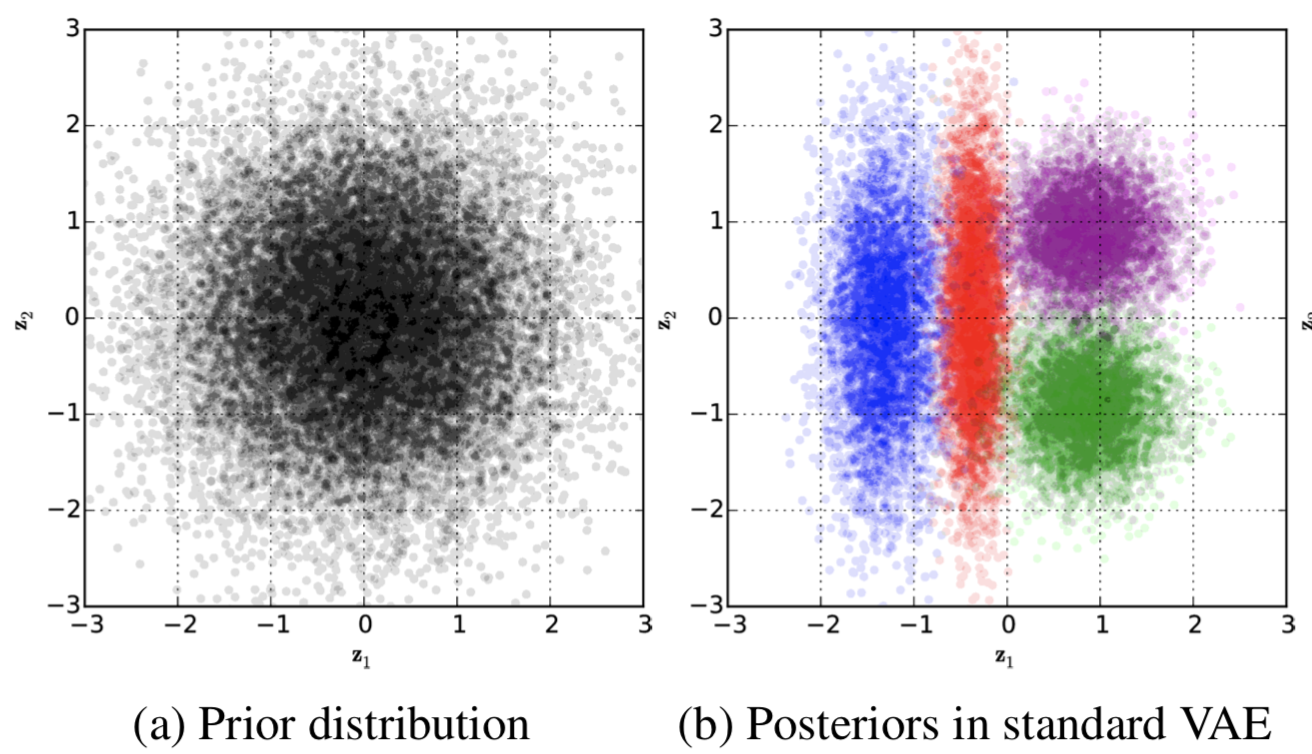
\includegraphics[width=0.65\linewidth]{figs/agg_posterior}
	\end{figure}
	\myfootnotewithlink{https://arxiv.org/abs/1505.05770}{Rezende D. J., Mohamed S. Variational Inference with Normalizing Flows, 2015} 
\end{frame}
%=======
\section{Learnable VAE prior}
%=======
\begin{frame}{VAE limitations}
	\begin{itemize}
		\item Poor generative distribution (decoder)
		\[
		p(\bx | \bz, \btheta) = \mathcal{N}(\bx| \bmu_{\btheta}(\bz), \bsigma^2_{\btheta}(\bz)) \quad \text{or } = \text{Softmax}(\bpi_{\btheta}(\bz)).
		\]
		\item Loose lower bound
		\[
		\log p(\bx | \btheta) - \mathcal{L}(q, \btheta) = (?).
		\]
		\item \textbf{Poor prior distribution}
		\[
		p(\bz) = \mathcal{N}(0, \mathbf{I}).
		\]
		\item Poor variational posterior distribution (encoder)
		\[
		q(\bz | \bx, \bphi) = \mathcal{N}(\bz| \bmu_{\bphi}(\bx), \bsigma^2_{\bphi}(\bx)).
		\]
	\end{itemize}
\end{frame}
%=======
\begin{frame}{Optimal VAE prior}
	\begin{itemize}
		\item Standard Gaussian $p(\bz) = \mathcal{N}(0, I)$ $\Rightarrow$ over-regularization;
		\item $p(\bz) = q_{\text{agg}}(\bz) = \frac{1}{n}\sum_{i=1}^n q(\bz | \bx_i)$ $\Rightarrow$ overfitting and highly expensive.
	\end{itemize}
	\vspace{-0.5cm}
	\begin{minipage}[t]{0.5\columnwidth}
		\begin{block}{Non learnable prior $p(\bz)$}
			\begin{figure}[h]
				\centering
				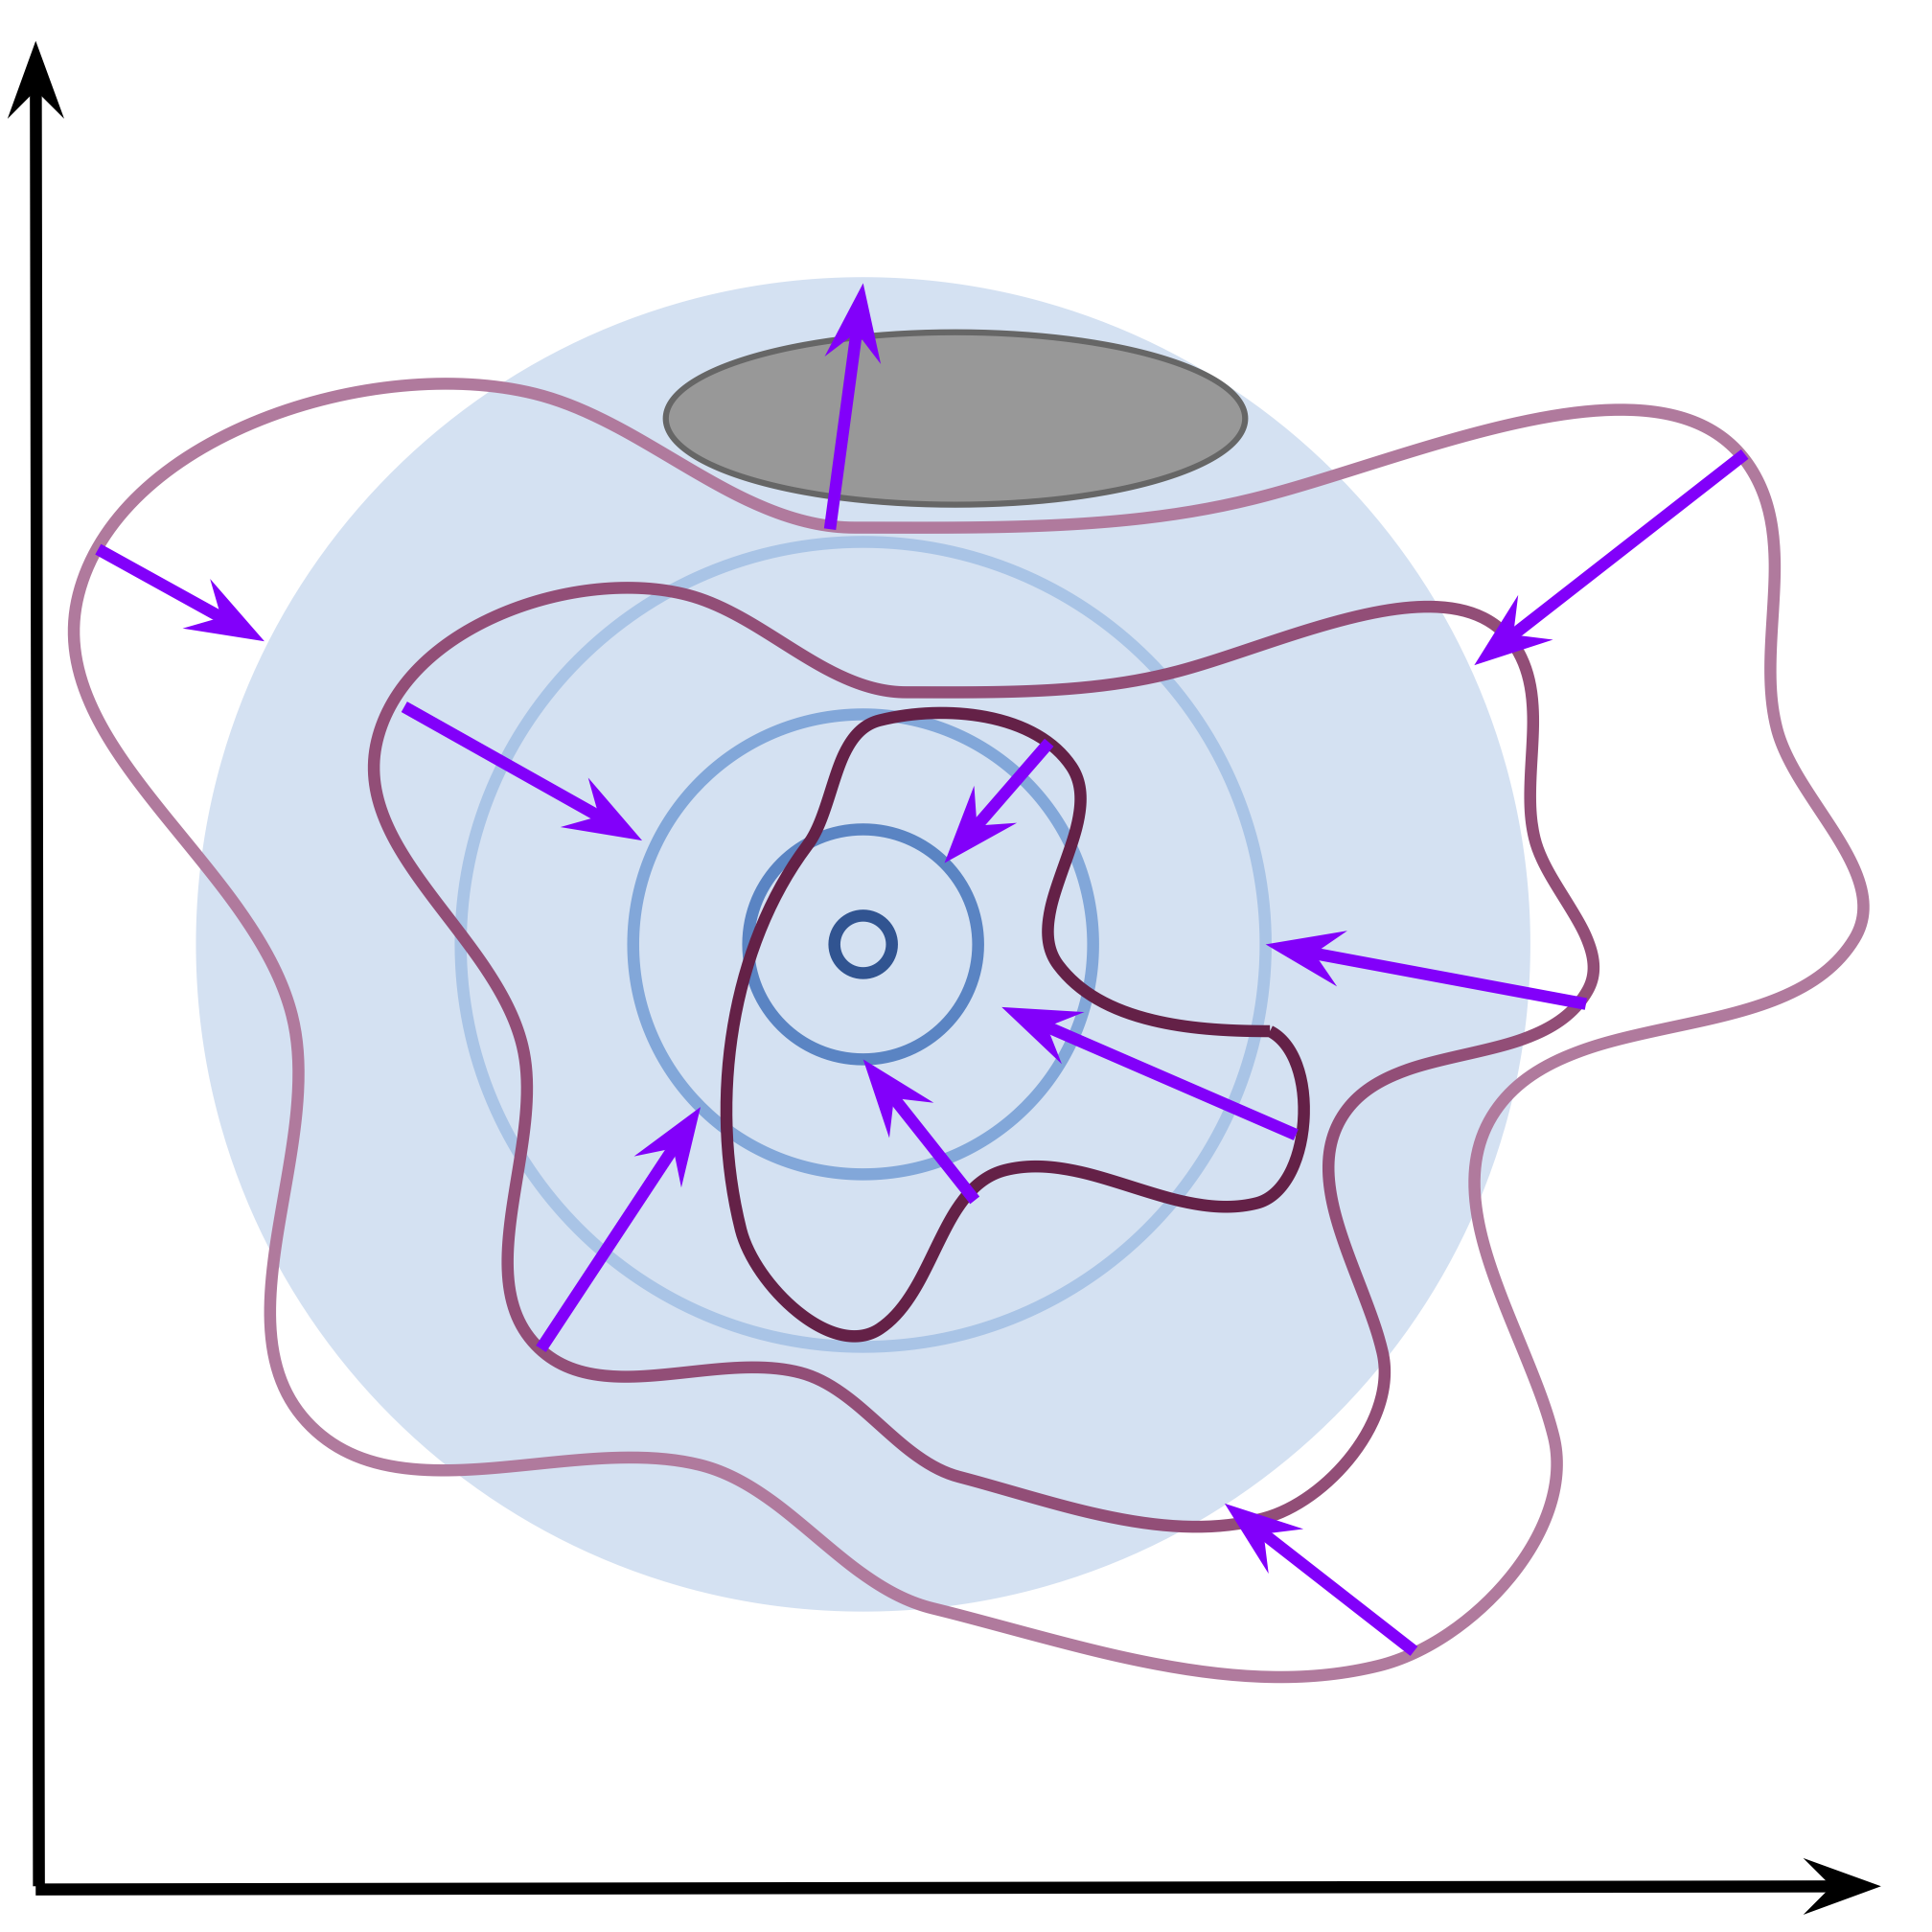
\includegraphics[width=0.6\linewidth]{figs/non_learnable_prior}
			\end{figure}
		\end{block}
	\end{minipage}%
	\begin{minipage}[t]{0.5\columnwidth}
		\begin{block}{Learnable prior $p(\bz | \blambda)$}
			\begin{figure}[h]
				\centering
				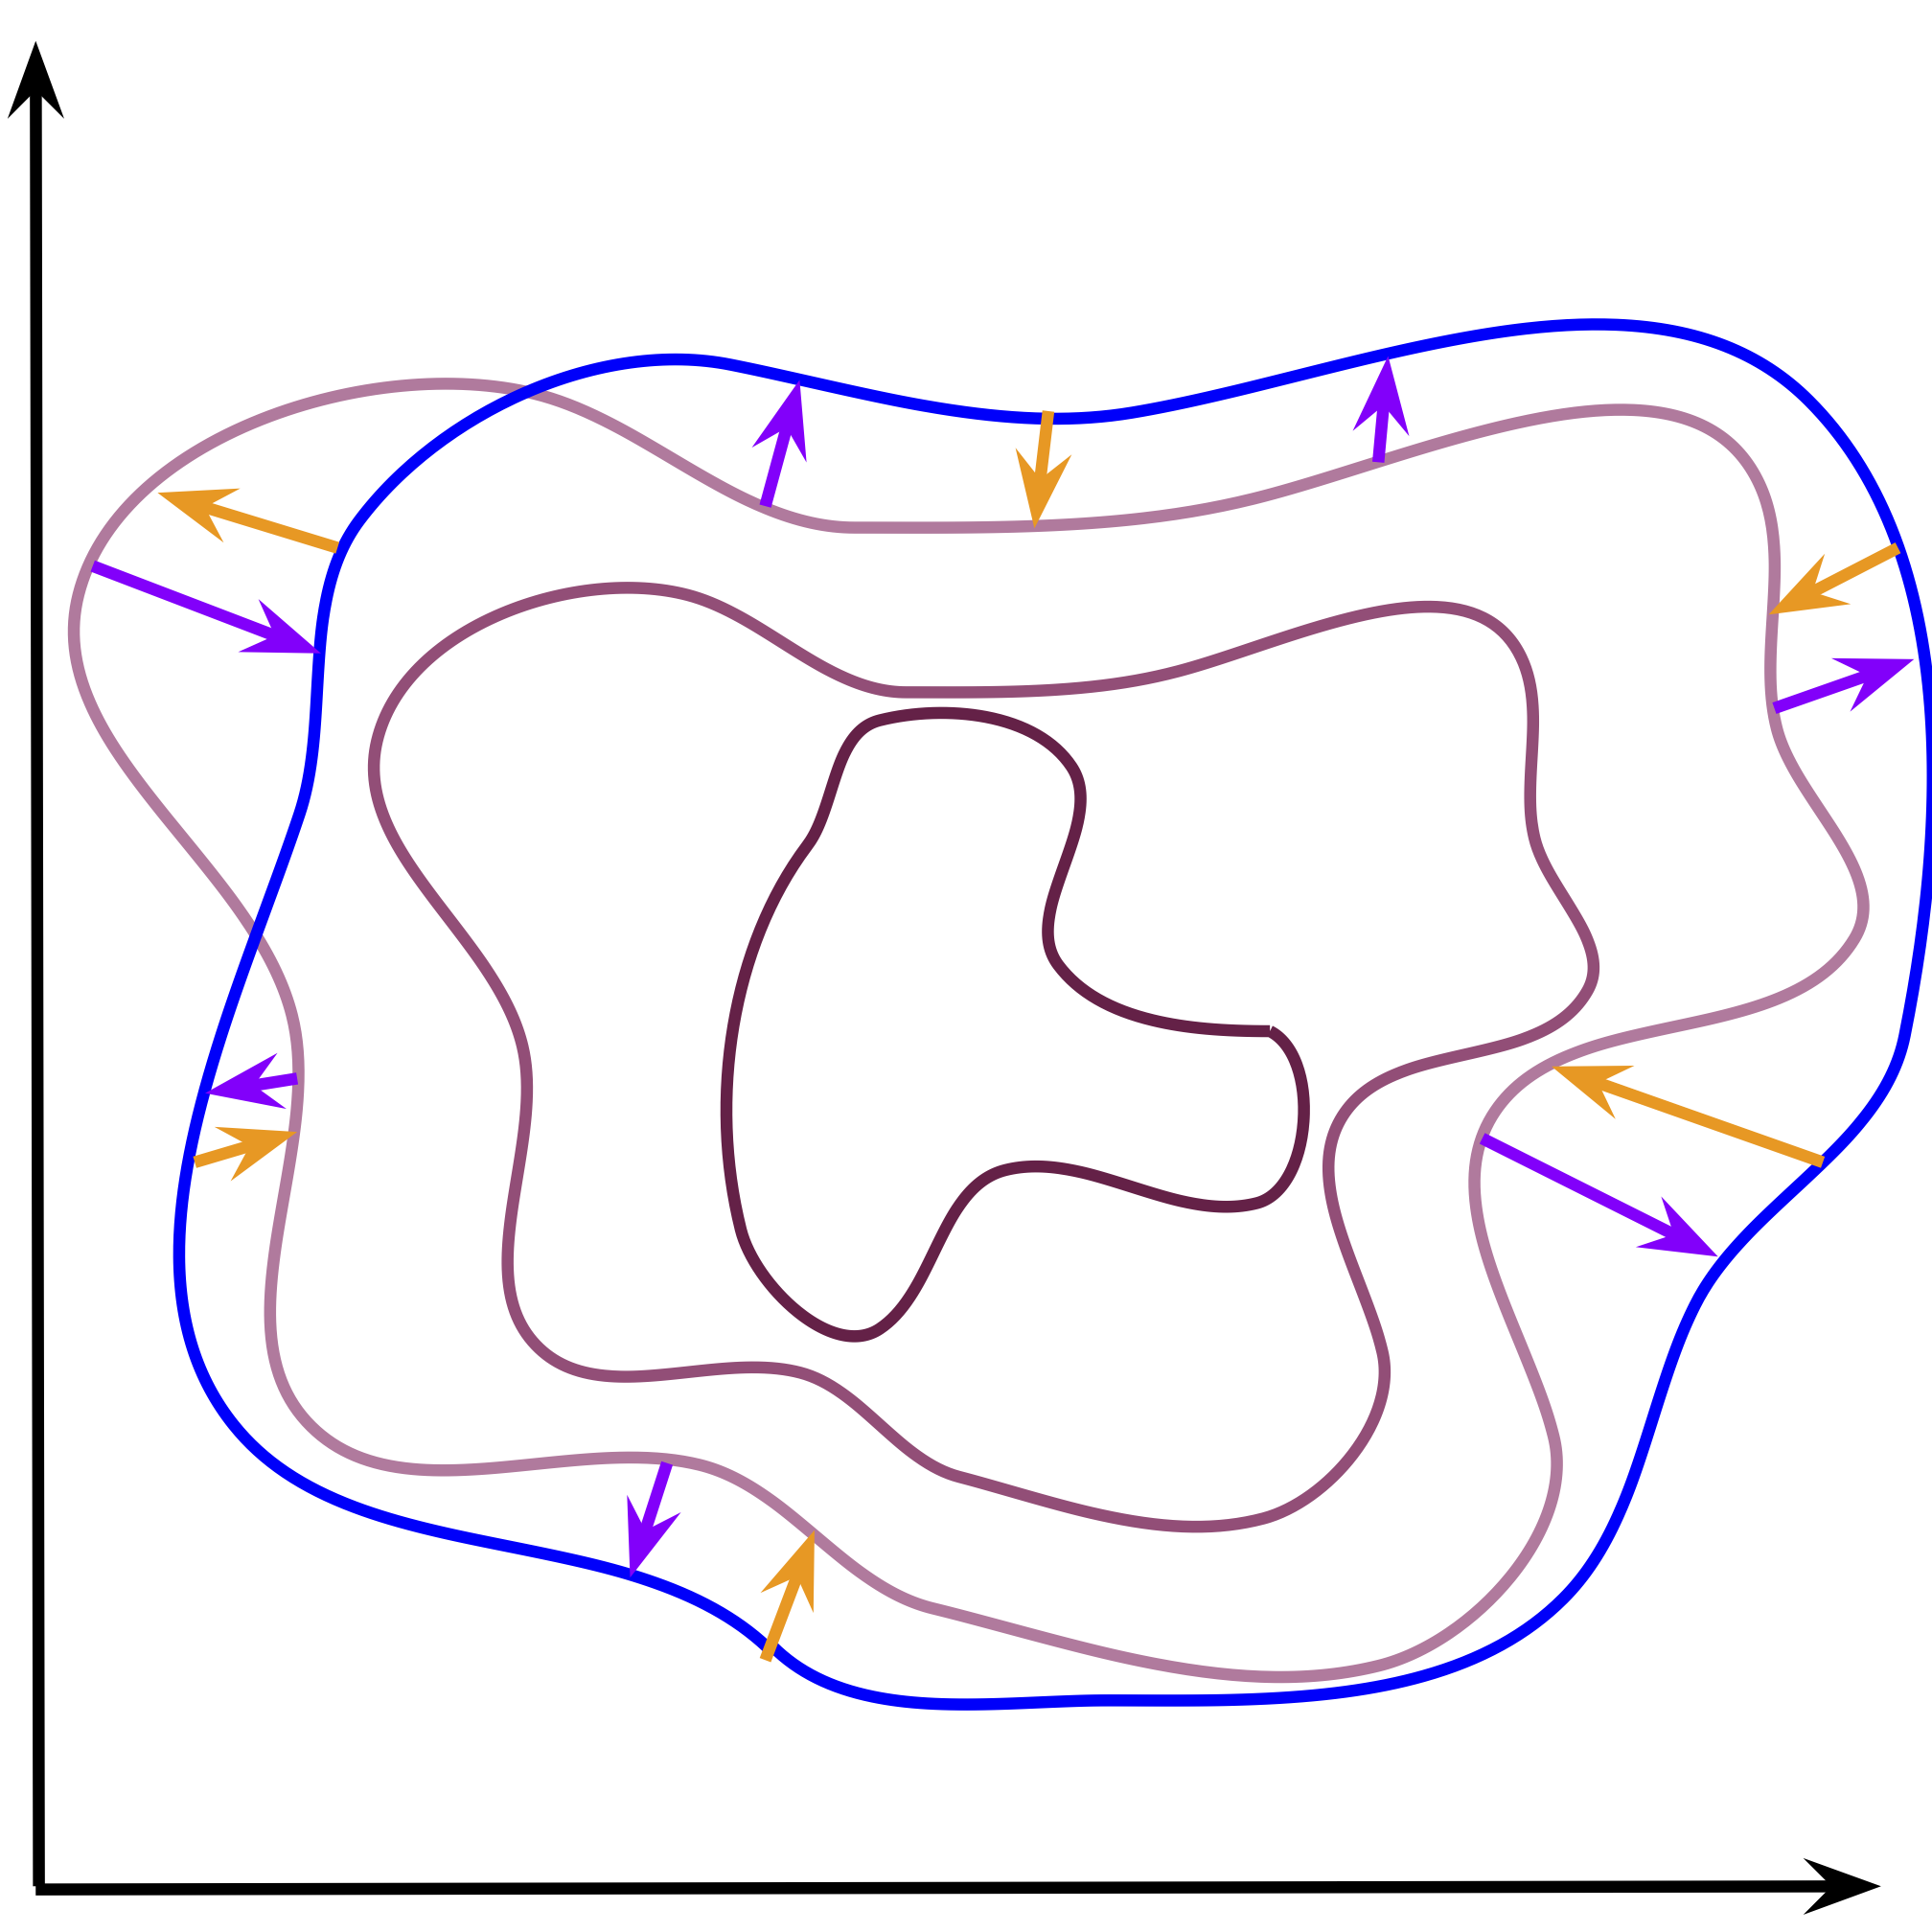
\includegraphics[width=0.6\linewidth]{figs/learnable_prior}
			\end{figure}
		\end{block}
	\end{minipage}
	\vspace{-0.4cm}
	\begin{block}{ELBO revisiting}
		\vspace{-0.3cm}
		\[
			\frac{1}{n}\sum_{i=1}^n \cL_i(q, \btheta) = \text{RL} - \text{MI} -  KL(q_{\text{agg}}(\bz) || {\color{teal}p(\bz | \blambda)})
		\]
		It is Forward KL with respect to $p(\bz | \blambda)$.
	\end{block}
	\myfootnotewithlink{https://jmtomczak.github.io/blog/7/7\_priors.html}{image credit: https://jmtomczak.github.io/blog/7/7\_priors.html}
\end{frame}
%=======
\begin{frame}{NF-based VAE prior}
	\begin{block}{NF model in latent space}
		\vspace{-0.5cm}
		\[
			\log p(\bz | \blambda) = \log p(\bz^*) + \log  \left | \det \left(\frac{d \bz^*}{d\bz}\right)\right| = \log p(f(\bz, \blambda)) + \log \left | \det (\bJ_f)\right| 
		\]
		\vspace{-0.3cm}
		\[
			\bz = g_{\blambda}(\bz^*) = f^{-1}_{\blambda}(\bz^*)
		\]
	\end{block}
	\vspace{-0.3cm}
	\begin{itemize}
		\item RealNVP with coupling layers.
		\item Autoregressive NF (fast $f_{\blambda}(\bz)$, slow $g_{\blambda}(\bz^*)$).
	\end{itemize}
	\begin{block}{ELBO with NF-based VAE prior}
		\vspace{-0.5cm}
		{\small
		\begin{multline*}
			\mathcal{L}(\bphi, \btheta) = \mathbb{E}_{q(\bz | \bx, \bphi)} \left[ \log p(\bx | \bz, \btheta) + {\color{violet}\log p(\bz | \blambda)} - \log q(\bz | \bx, \bphi) \right] \\
				= \mathbb{E}_{q(\bz | \bx, \bphi)} \Bigl[ \log p(\bx | \bz, \btheta) + \underbrace{ \Bigl({\color{violet} \log p(f_{\blambda}(\bz)) + \log \left| \det (\bJ_f) \right|} \Bigr) }_{\text{NF-based prior}} - \log q(\bz | \bx, \bphi) \Bigr] 
		\end{multline*}
		}
	\end{block}
	\myfootnotewithlink{https://arxiv.org/abs/1611.02731}{Chen X. et al. Variational Lossy Autoencoder, 2016}
\end{frame}
%=======
\section{Discrete VAE latent representations}
%=======
\begin{frame}{Discrete VAE latents}
	\begin{block}{Motivation}
		\begin{itemize}
			\item Previous VAE models had \textbf{continuous} latent variables $\bz$.
			\item \textbf{Discrete} representations $\bz$ are potentially a more natural fit for many of the modalities.
			\item Powerful autoregressive models (like PixelCNN) have been developed for modelling distributions over discrete variables.
			\item All cool transformer-like models work with discrete tokens.
		\end{itemize}
	\end{block}
	\begin{block}{ELBO}
		\vspace{-0.3cm}
		\[
		\mathcal{L} (\bphi, \btheta)  = \mathbb{E}_{q(\bz | \bx, \bphi)} \log p(\bx | \bz , \btheta) - KL(q(\bz| \bx, \bphi) || p(\bz)) \rightarrow \max_{\bphi, \btheta}.
		\]
		\vspace{-0.5cm}
	\end{block}
	\begin{itemize}
		\item Reparametrization trick to get unbiased gradients.
		\item Normal assumptions for $q(\bz | \bx, \bphi)$ and $p(\bz)$ to compute KL analytically.
	\end{itemize}
\end{frame}
%=======
\begin{frame}{Discrete VAE latents}
	\begin{block}{Assumptions}
		\begin{itemize}
			\item Define dictionary (word book) space $\{\be_k\}_{k=1}^K$, where $\be_k \in \bbR^C$, $K$ is the size of the dictionary.
			\item Let $c \sim \text{Categorical}(\bpi)$, where 
			\vspace{-0.6cm}
			\[
			\bpi = (\pi_1, \dots, \pi_K), \quad \pi_k = P(c = k), \quad \sum_{k=1}^K \pi_k = 1.
			\]
			\vspace{-0.6cm}
			\item Let VAE model has discrete latent representation $c$ with prior $p(c) = \text{Uniform}\{1, \dots, K\}$.
		\end{itemize}
	\end{block}
	\vspace{-0.3cm}
	\begin{block}{How it should work?}
		\begin{itemize}
			\item Our variational posterior $q(c | \bx, \bphi) = \text{Categorical}(\bpi_{\bphi}(\bx))$ (encoder) outputs discrete probabilities vector.
			\item We sample $c^*$ from $q(c | \bx, \bphi)$ (reparametrization trick analogue).
			\item Our generative distribution $p(\bx | \be_{c^*}, \btheta)$ (decoder).
		\end{itemize}
	\end{block}
\end{frame}
%=======
\begin{frame}{Discrete VAE latents}
	\begin{block}{ELBO}
		\vspace{-0.5cm}
		\[
		\mathcal{L} (\bphi, \btheta)  = \mathbb{E}_{q(c | \bx, \bphi)} \log p(\bx | c, \btheta) - KL(q(c| \bx, \bphi) || p(c)) \rightarrow \max_{\bphi, \btheta}.
		\]
		\vspace{-0.5cm}
	\end{block}
	\begin{block}{KL term}
		\vspace{-0.8cm}
		\begin{multline*}
			KL(q(c| \bx, \bphi) || p(c)) = \sum_{k=1}^K q(k | \bx, \bphi) \log \frac{q(k | \bx, \bphi)}{p(k)} = 
			\\ = \color{violet}{\sum_{k=1}^K q(k | \bx, \bphi) \log q(k | \bx, \bphi)}  \color{teal}{- \sum_{k=1}^K q(k | \bx, \bphi) \log p(k)}  = \\ = \color{violet}{- H(q(c | \bx, \bphi))} + \color{teal}{\log K}. 
		\end{multline*}
		\vspace{-0.6cm}
	\end{block}
	\begin{itemize}
		\item Is it possible to make reparametrization trick? (we sample from discrete distribution now!).
		\item Entropy term should be estimated.
	\end{itemize}
\end{frame}
%=======
\subsection{Vector quantization}
%=======
\begin{frame}{Vector quantization}
	\begin{block}{Quantized representation}
		$\bz_q \in \bbR^{C}$  for $\bz \in \bbR^C$ is defined by a nearest neighbor look-up using the shared dictionary space
		\vspace{-0.3cm}
		\[
		\bz_q = \be_{k^*}, \quad \text{where } k^* = \argmin_k \| \bz - \be_k \|.
		\] 
		\vspace{-0.7cm}
	\end{block}
	\begin{itemize}
		\item Let our encoder outputs continuous representation $\bz$. 
		\item Quantization will give us the discrete distribution $q(c | \bx, \bphi)$.
	\end{itemize}
	\vspace{-0.2cm}
	\begin{block}{Quantization procedure}
		If we have tensor with the spatial dimensions we apply the quantization for each of $W \times H$ locations.
		\begin{minipage}[t]{0.65\columnwidth}
			\begin{figure}
				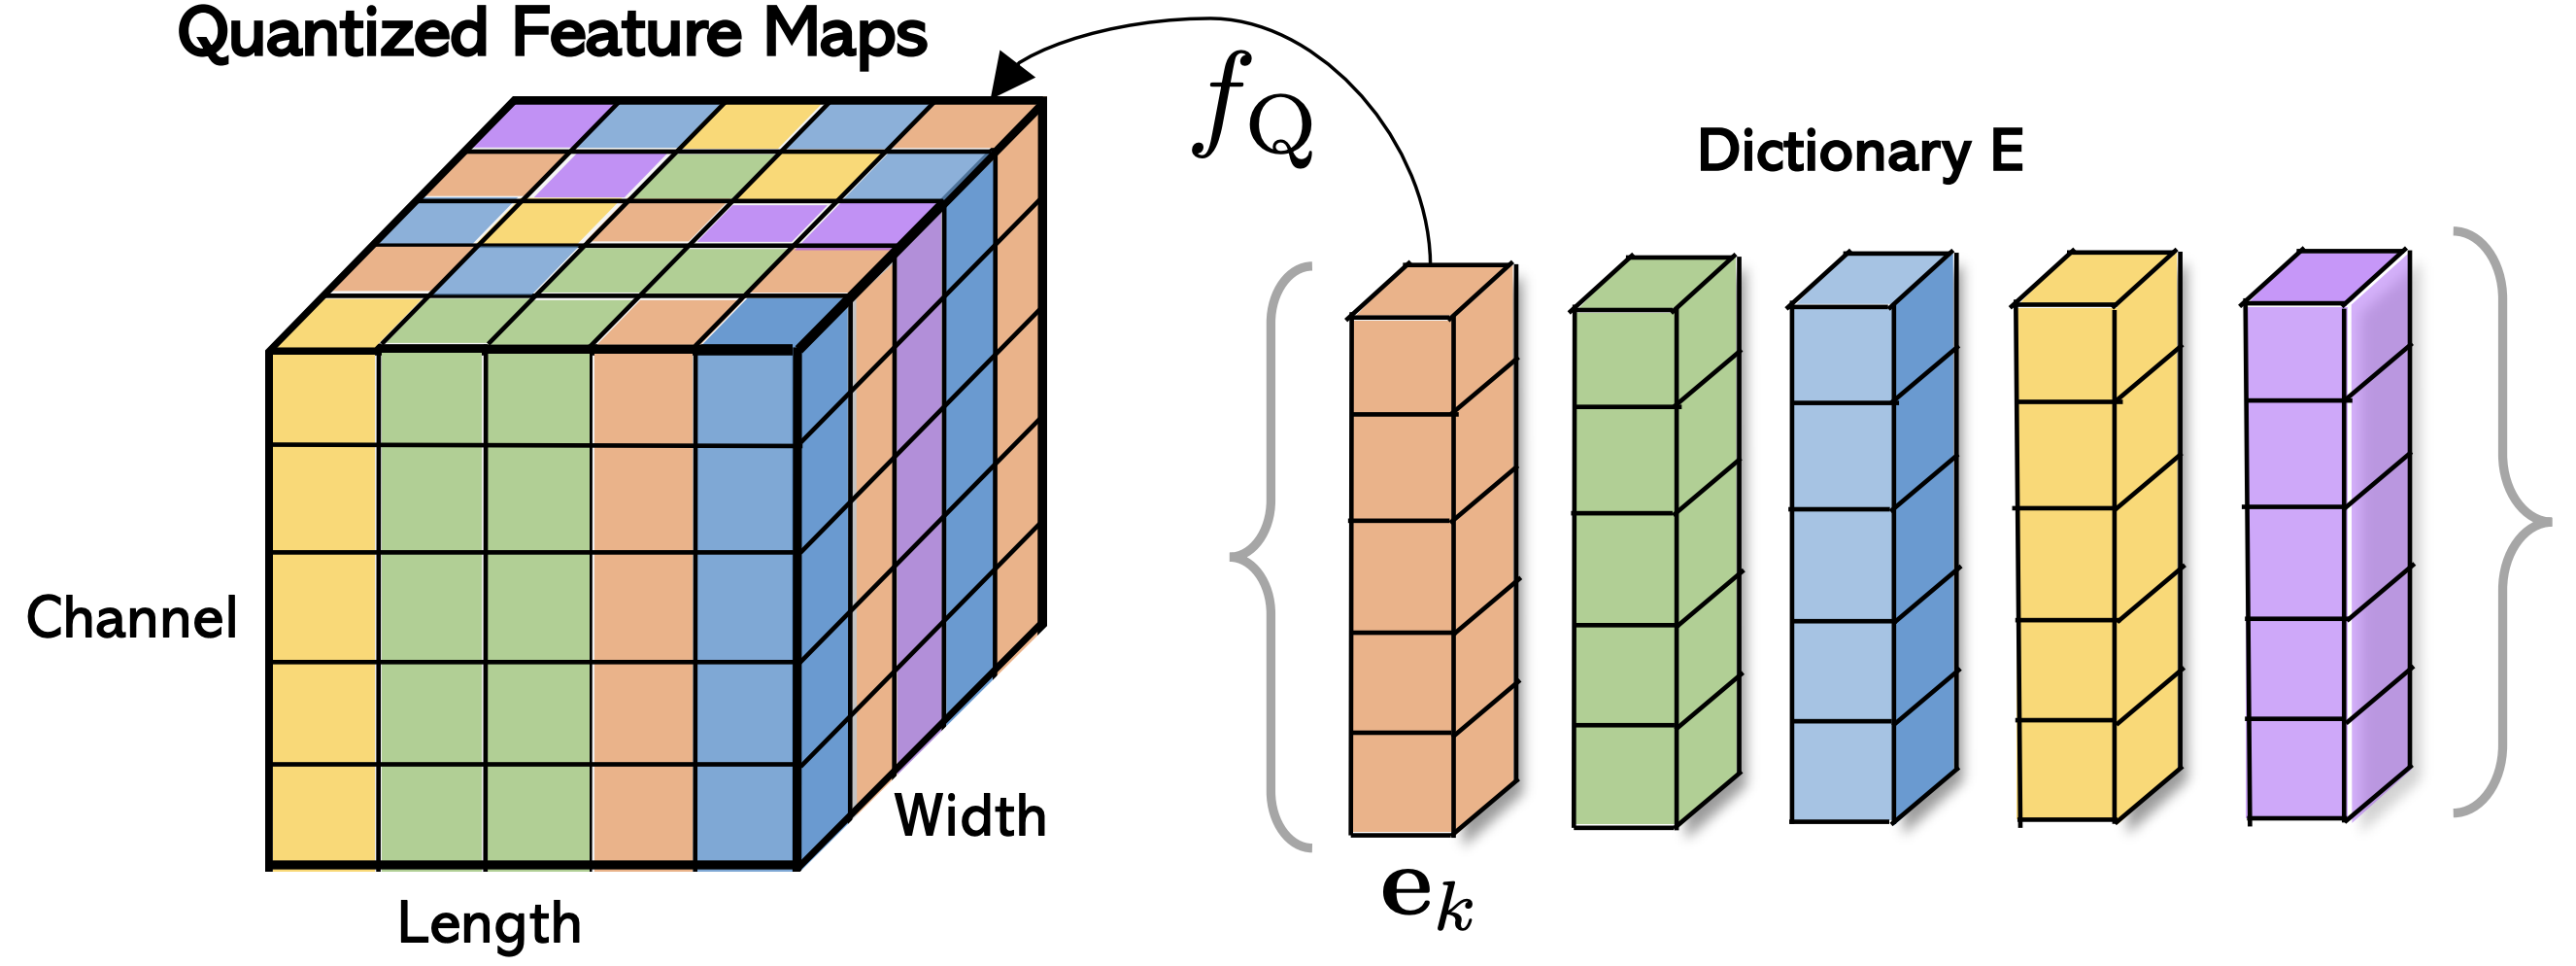
\includegraphics[width=0.8\linewidth]{figs/fqgan_cnn.png}
			\end{figure}
		\end{minipage}%
		\begin{minipage}[t]{0.35\columnwidth}
			\begin{figure}
				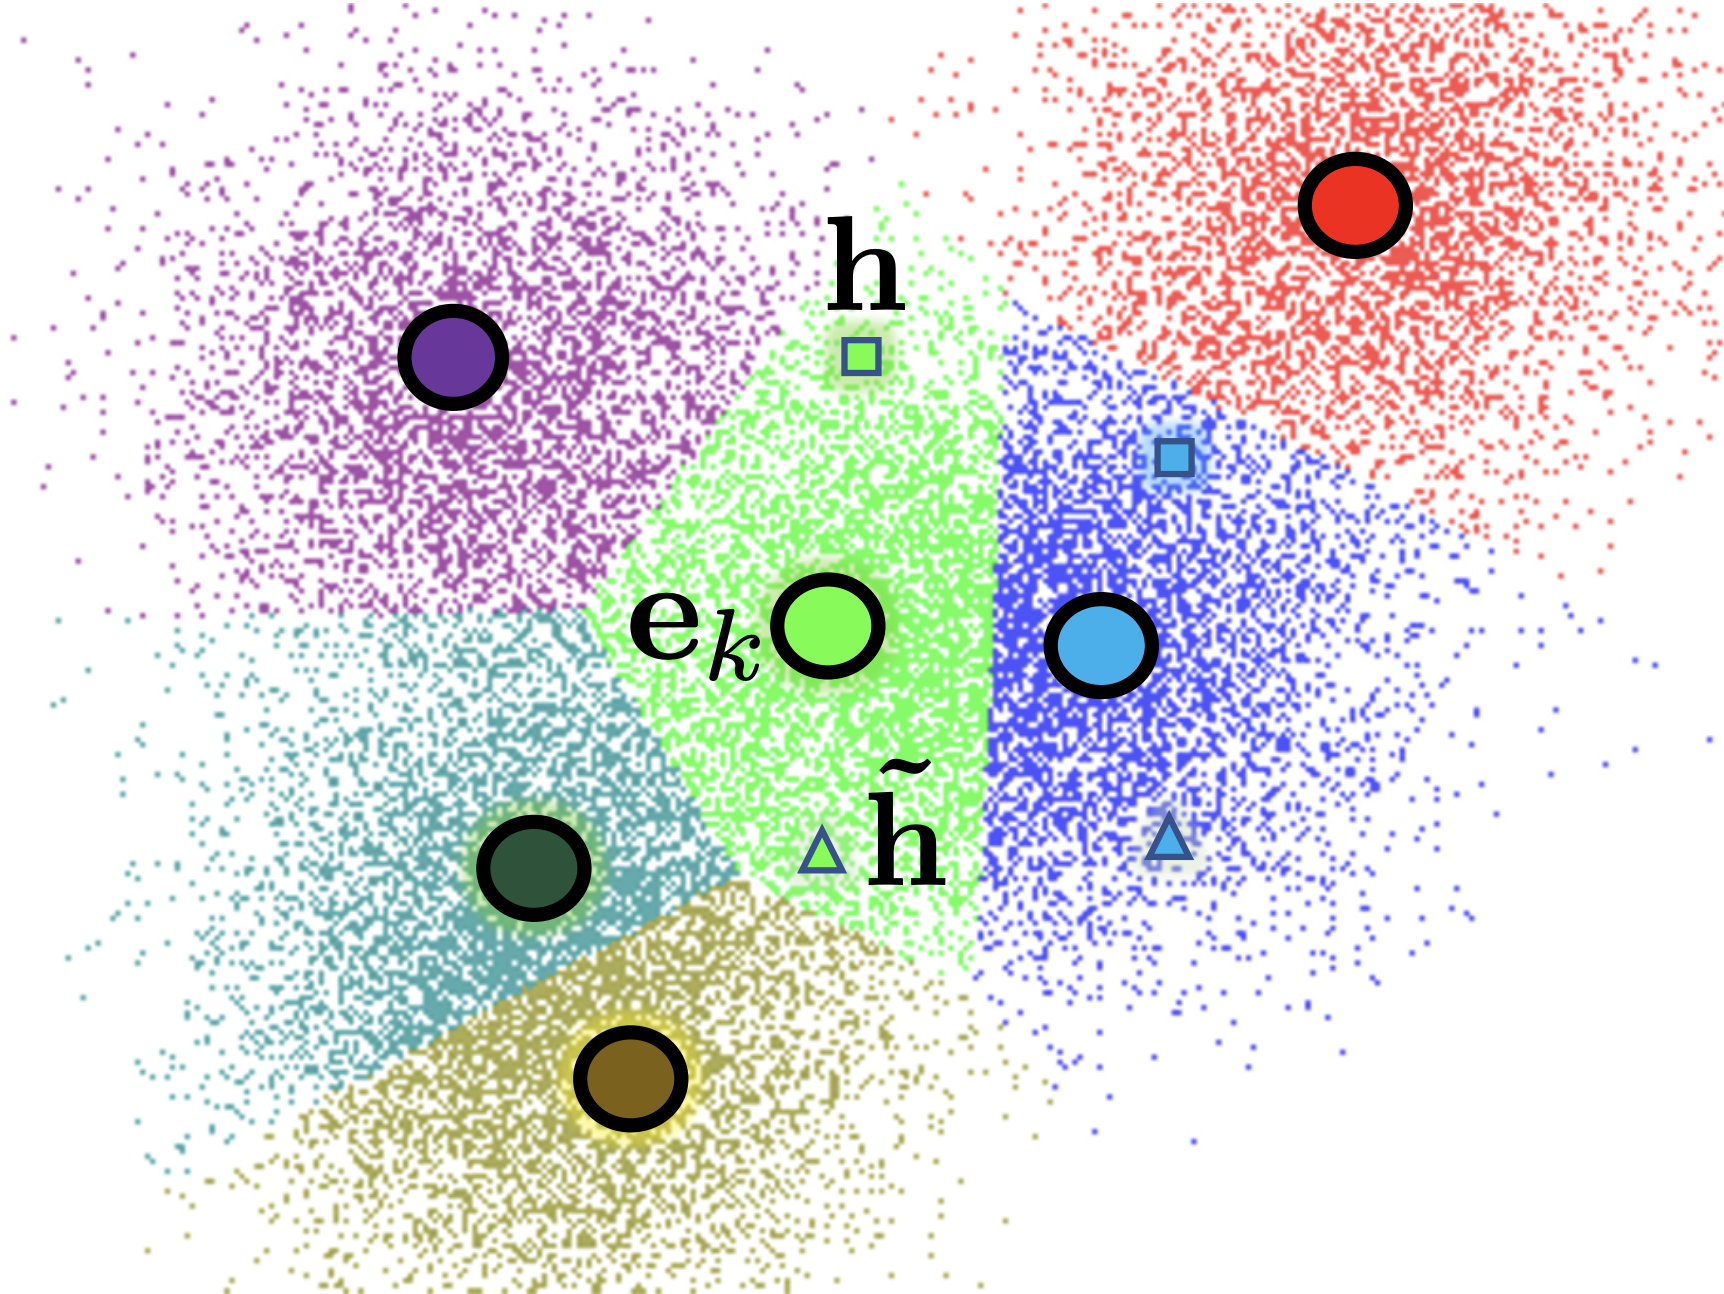
\includegraphics[width=0.7\linewidth]{figs/fqgan_lookup}
			\end{figure}
		\end{minipage}
	\end{block}
	\myfootnotewithlink{https://arxiv.org/abs/2004.02088}{Zhao Y. et al. Feature Quantization Improves GAN Training, 2020} 
\end{frame}
%=======
\begin{frame}{Vector Quantized VAE (VQ-VAE)}
	Let VAE latent variable $\bc \in \{1, \dots, K\}^{W \times H}$ is the discrete with spatial-independent variational posterior and prior distributions  
	\vspace{-0.3cm}
	\[
	q(\bc | \bx, \bphi) = \prod_{i=1}^W \prod_{j=1}^H q(c_{ij} | \bx, \bphi); \quad p(\bc) = \prod_{i=1}^W \prod_{j=1}^H \text{Uniform}\{1, \dots, K\}.
	\]
	Let $\bz_e = \text{NN}_{e, \bphi}(\bx) \in \bbR^{W \times H \times C}$ is the encoder output.
	\begin{block}{Deterministic variational posterior}
		\vspace{-0.6cm}
		\[
		q(c_{ij} = k^* | \bx, \bphi) = \begin{cases}
			1 , \quad \text{for } k^* = \argmin_k \| [\bz_e]_{ij} - \be_k \|; \\
			0, \quad \text{otherwise}.
		\end{cases}
		\]
		$KL(q(c| \bx, \bphi) || p(c))$ term in ELBO is constant, entropy of the posterior is zero.
		\[
		KL(q(c | \bx, \bphi) || p(c)) = - H(q(c | \bx, \bphi)) + \log K = \log K. 
		\]
	\end{block}
	
	\myfootnotewithlink{https://arxiv.org/abs/1711.00937}{Oord A., Vinyals O., Kavukcuoglu K. Neural Discrete Representation Learning, 2017} 
\end{frame}
%=======
\begin{frame}{Vector Quantized VAE (VQ-VAE)}
	\begin{block}{ELBO}
		\vspace{-0.6cm}
		\[
		\mathcal{L} (\bphi, \btheta)  = \mathbb{E}_{q(c | \bx, \bphi)} \log p(\bx | \be_{c} , \btheta) - \log K =  \log p(\bx | \bz_q, \btheta) - \log K,
		\]
		where $\bz_q = \be_{k^*}$, $k^* = \argmin_k \| \bz_e - \be_k \|$.
	\end{block}
	\begin{figure}
		\centering
		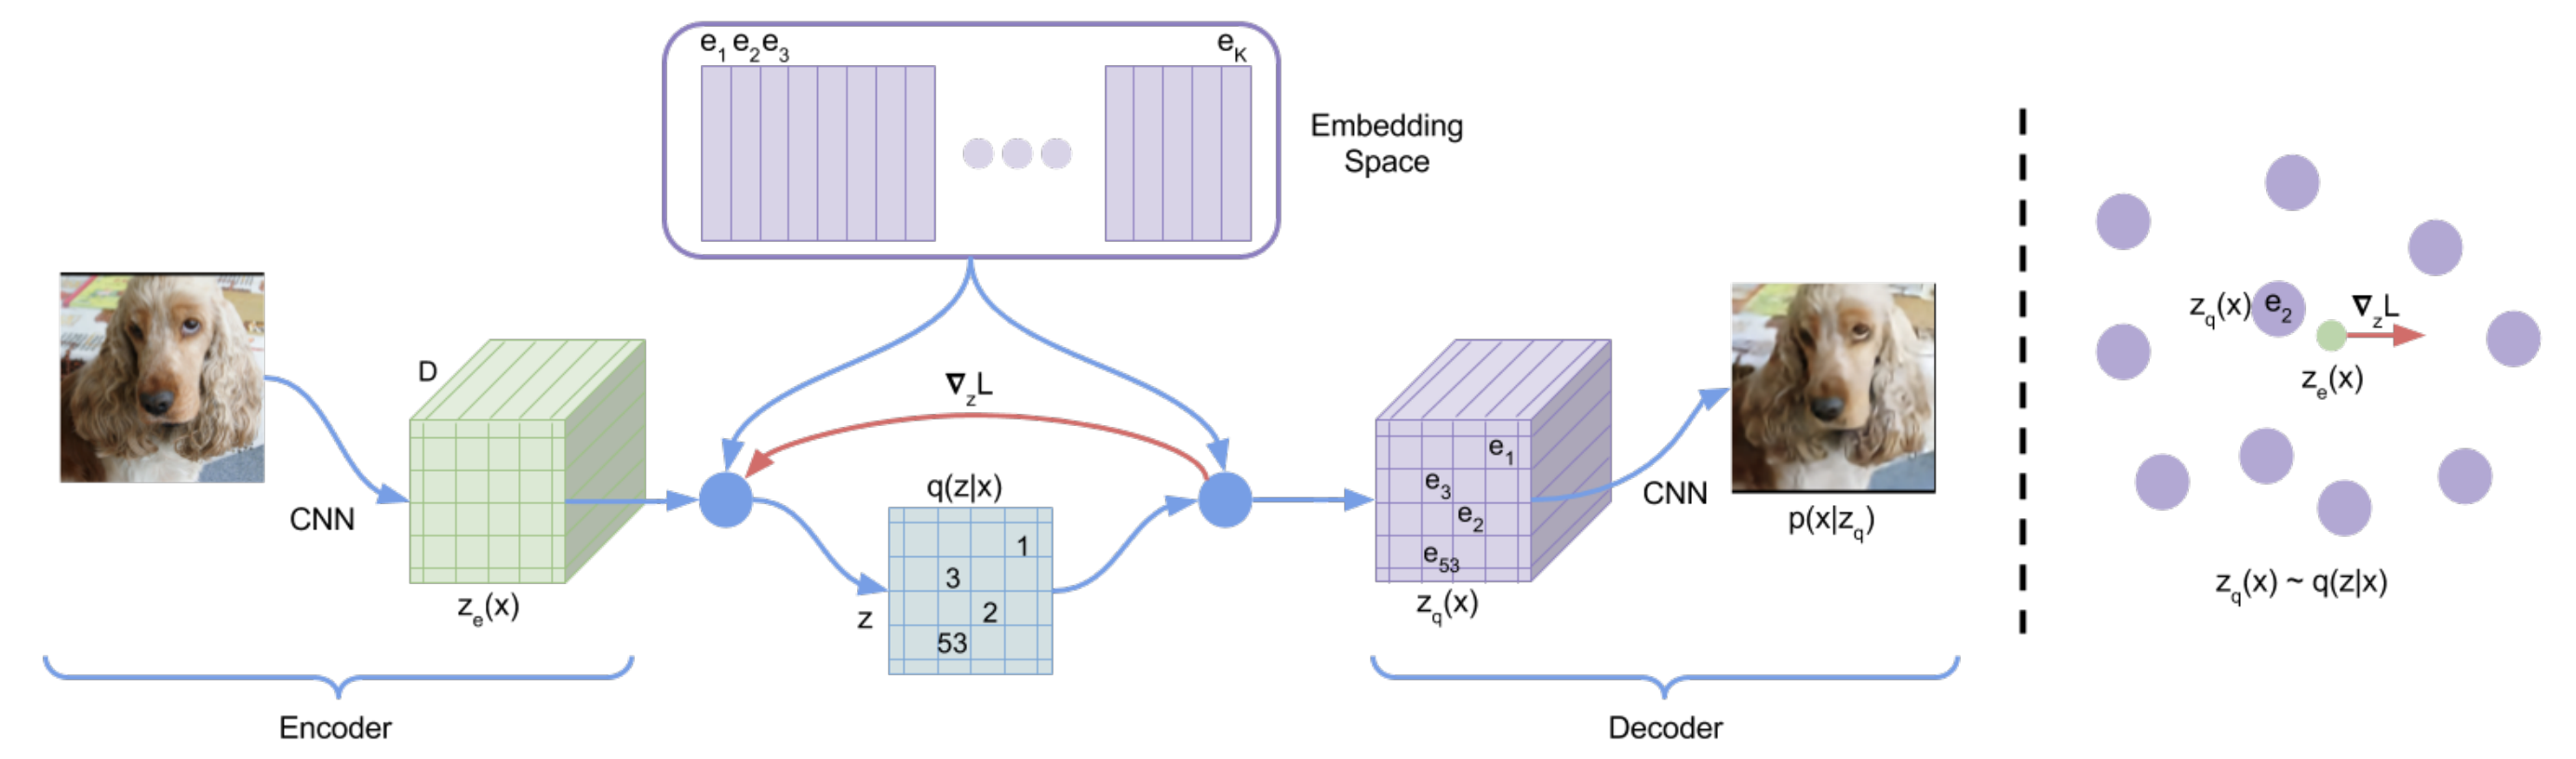
\includegraphics[width=0.85\linewidth]{figs/vqvae}
	\end{figure}
	\textbf{Problem:} $\argmin$ is not differentiable.
	\begin{block}{Straight-through gradient estimation}
		\vspace{-0.6cm}
		\[
		\frac{\partial \log p(\bx | \bz_q , \btheta)}{\partial \bphi} = \frac{\partial \log p(\bx | \bz_q, \btheta)}{\partial \bz_q} \cdot {\color{red}\frac{\partial \bz_q}{\partial \bphi}} \approx \frac{\partial \log p(\bx | \bz_q, \btheta)}{\partial \bz_q} \cdot \frac{\partial \bz_e}{\partial \bphi}
		\]
	\end{block}
	\myfootnotewithlink{https://arxiv.org/abs/1711.00937}{Oord A., Vinyals O., Kavukcuoglu K. Neural Discrete Representation Learning, 2017} 
\end{frame}
%=======
\begin{frame}{Vector Quantized VAE-2  (VQ-VAE-2)}
	\begin{block}{Samples 1024x1024}
		\vspace{-0.2cm}
		\begin{figure}
			\centering
			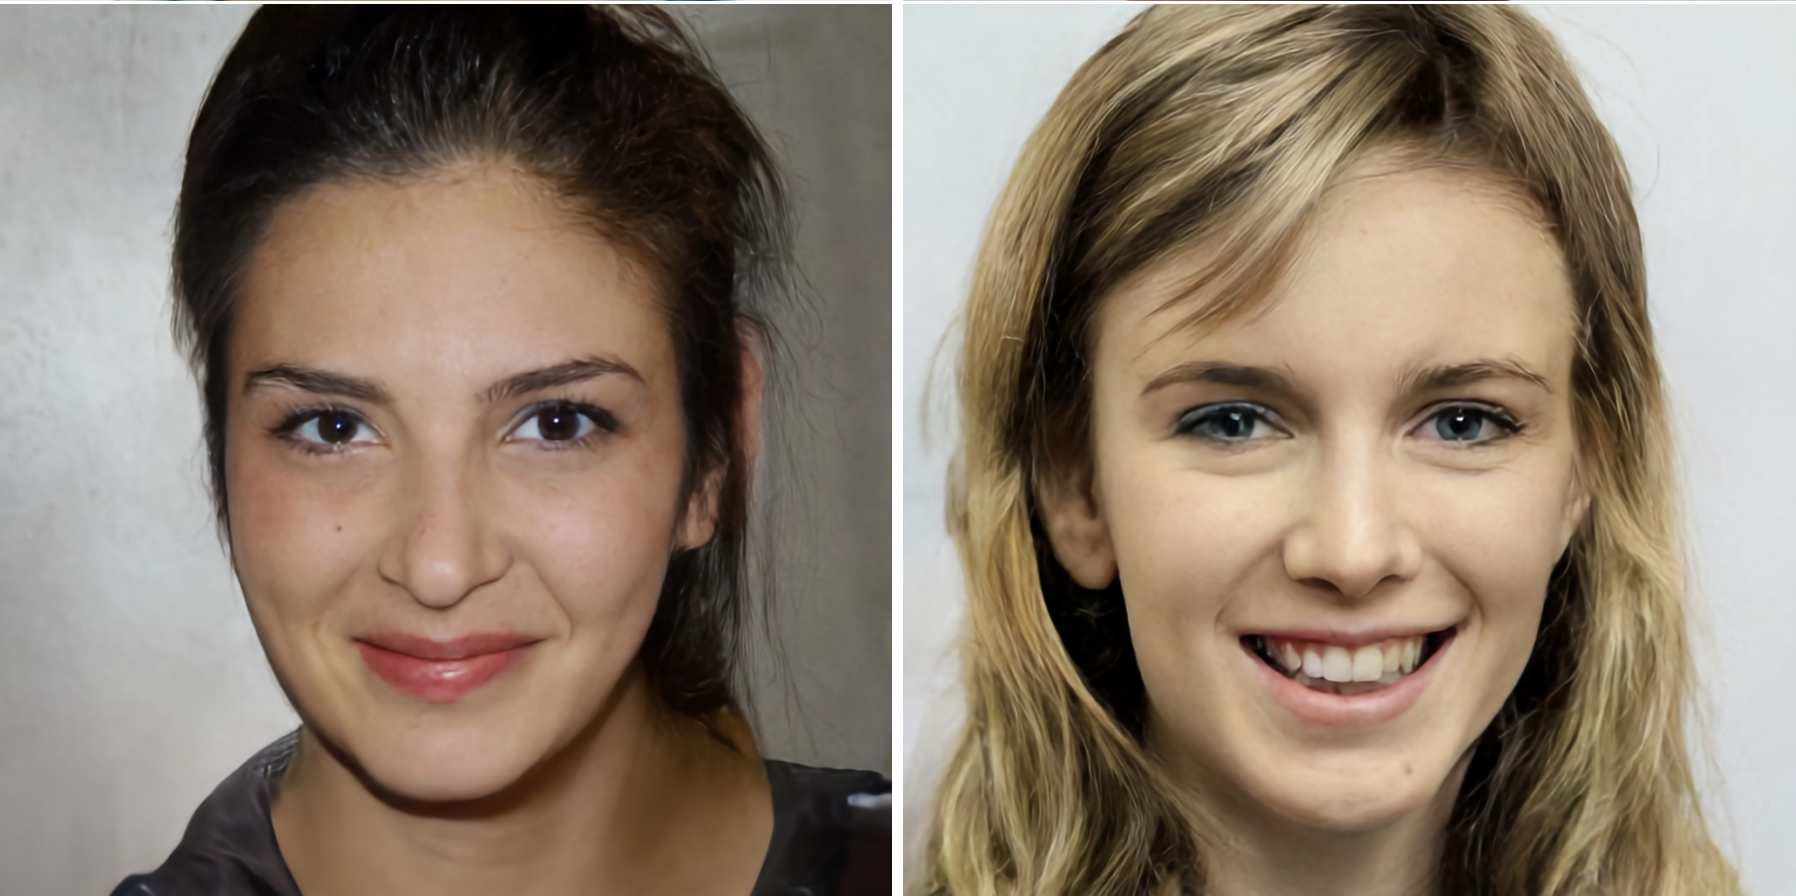
\includegraphics[width=0.63\linewidth]{figs/vqvae2_faces}
		\end{figure}
	\end{block}
	\vspace{-0.6cm}
	\begin{block}{Samples diversity}
		\vspace{-0.2cm}
		\begin{figure}
			\centering
			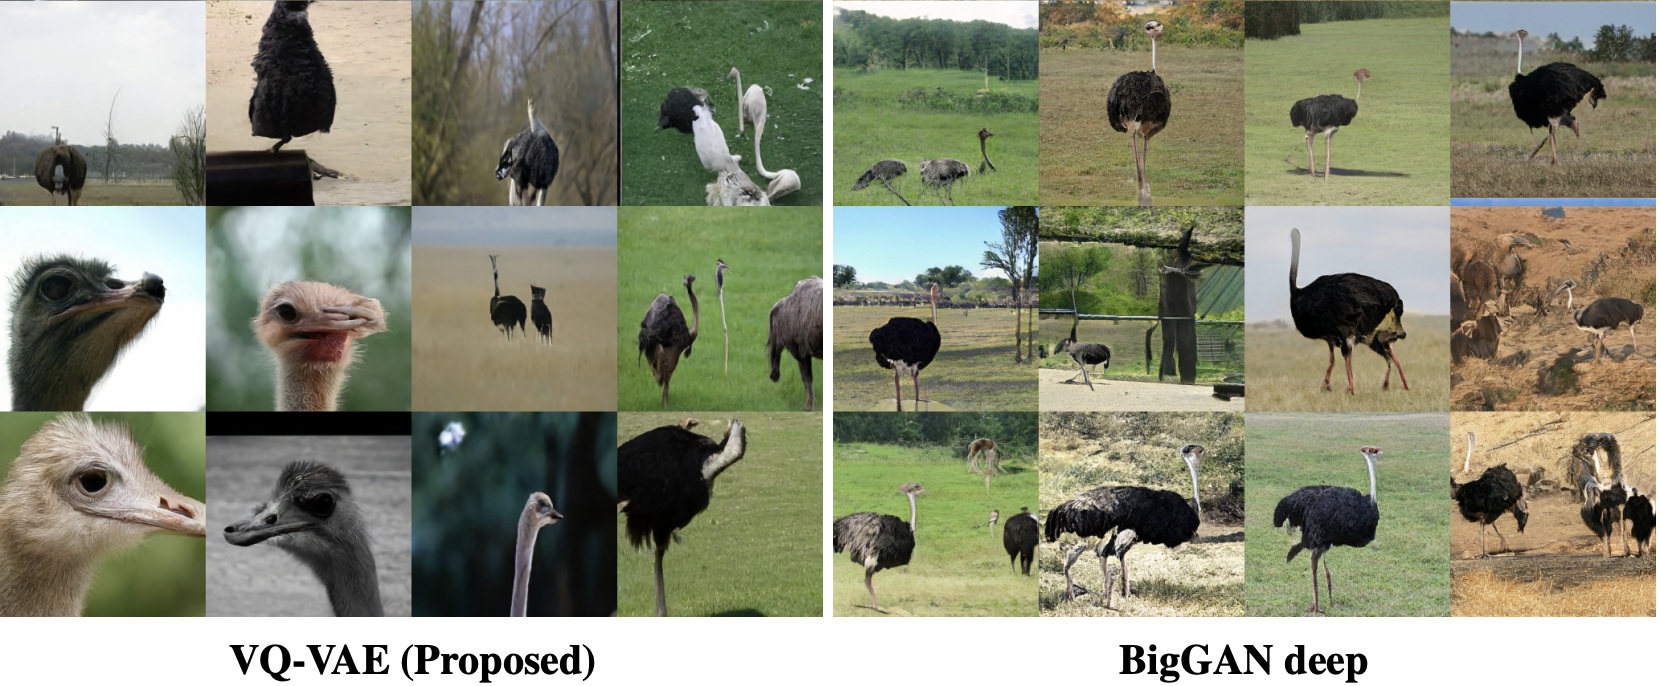
\includegraphics[width=0.65\linewidth]{figs/vqvae2_diversity}
		\end{figure}
	\end{block}
	\myfootnotewithlink{https://arxiv.org/abs/1906.00446}{Razavi A., Oord A., Vinyals O. Generating Diverse High-Fidelity Images with VQ-VAE-2, 2019} 
\end{frame}
%=======
\begin{frame}{Summary}
	\begin{itemize}
		\item The ELBO surgery reveals insights about a prior distribution in VAE. The optimal prior is the aggregated posterior.
		\vfill
		\item We could use NF-based prior in VAE (even autoregressive).
		\vfill
		\item Discrete VAE latents is a natural idea, but we have to avoid non-differentiable sampling operation.
		\vfill		
		\item Vector Quantization is the way to create VAE with discrete latent space and deterministic variational posterior. 
		\vfill
		\item Straight-through gradient ignores quantize operation in backprop.
	\end{itemize}
\end{frame}

\end{document} 
